\documentclass{article}

\usepackage{graphicx}
\usepackage{tikz}
\usepackage{tikzsymbols}
\usetikzlibrary{calc,patterns,shapes.geometric}
\pagestyle{empty}
\usepackage[margin=0pt]{geometry}
\geometry{papersize={14in,12in}}

\def\centerarc[#1](#2)(#3:#4:#5){\draw[#1] ($(#2)+({#5*cos(#3)},{#5*sin(#3)})$) arc (#3:#4:#5);}

\begin{document}
	\begin{figure}
		\centering
		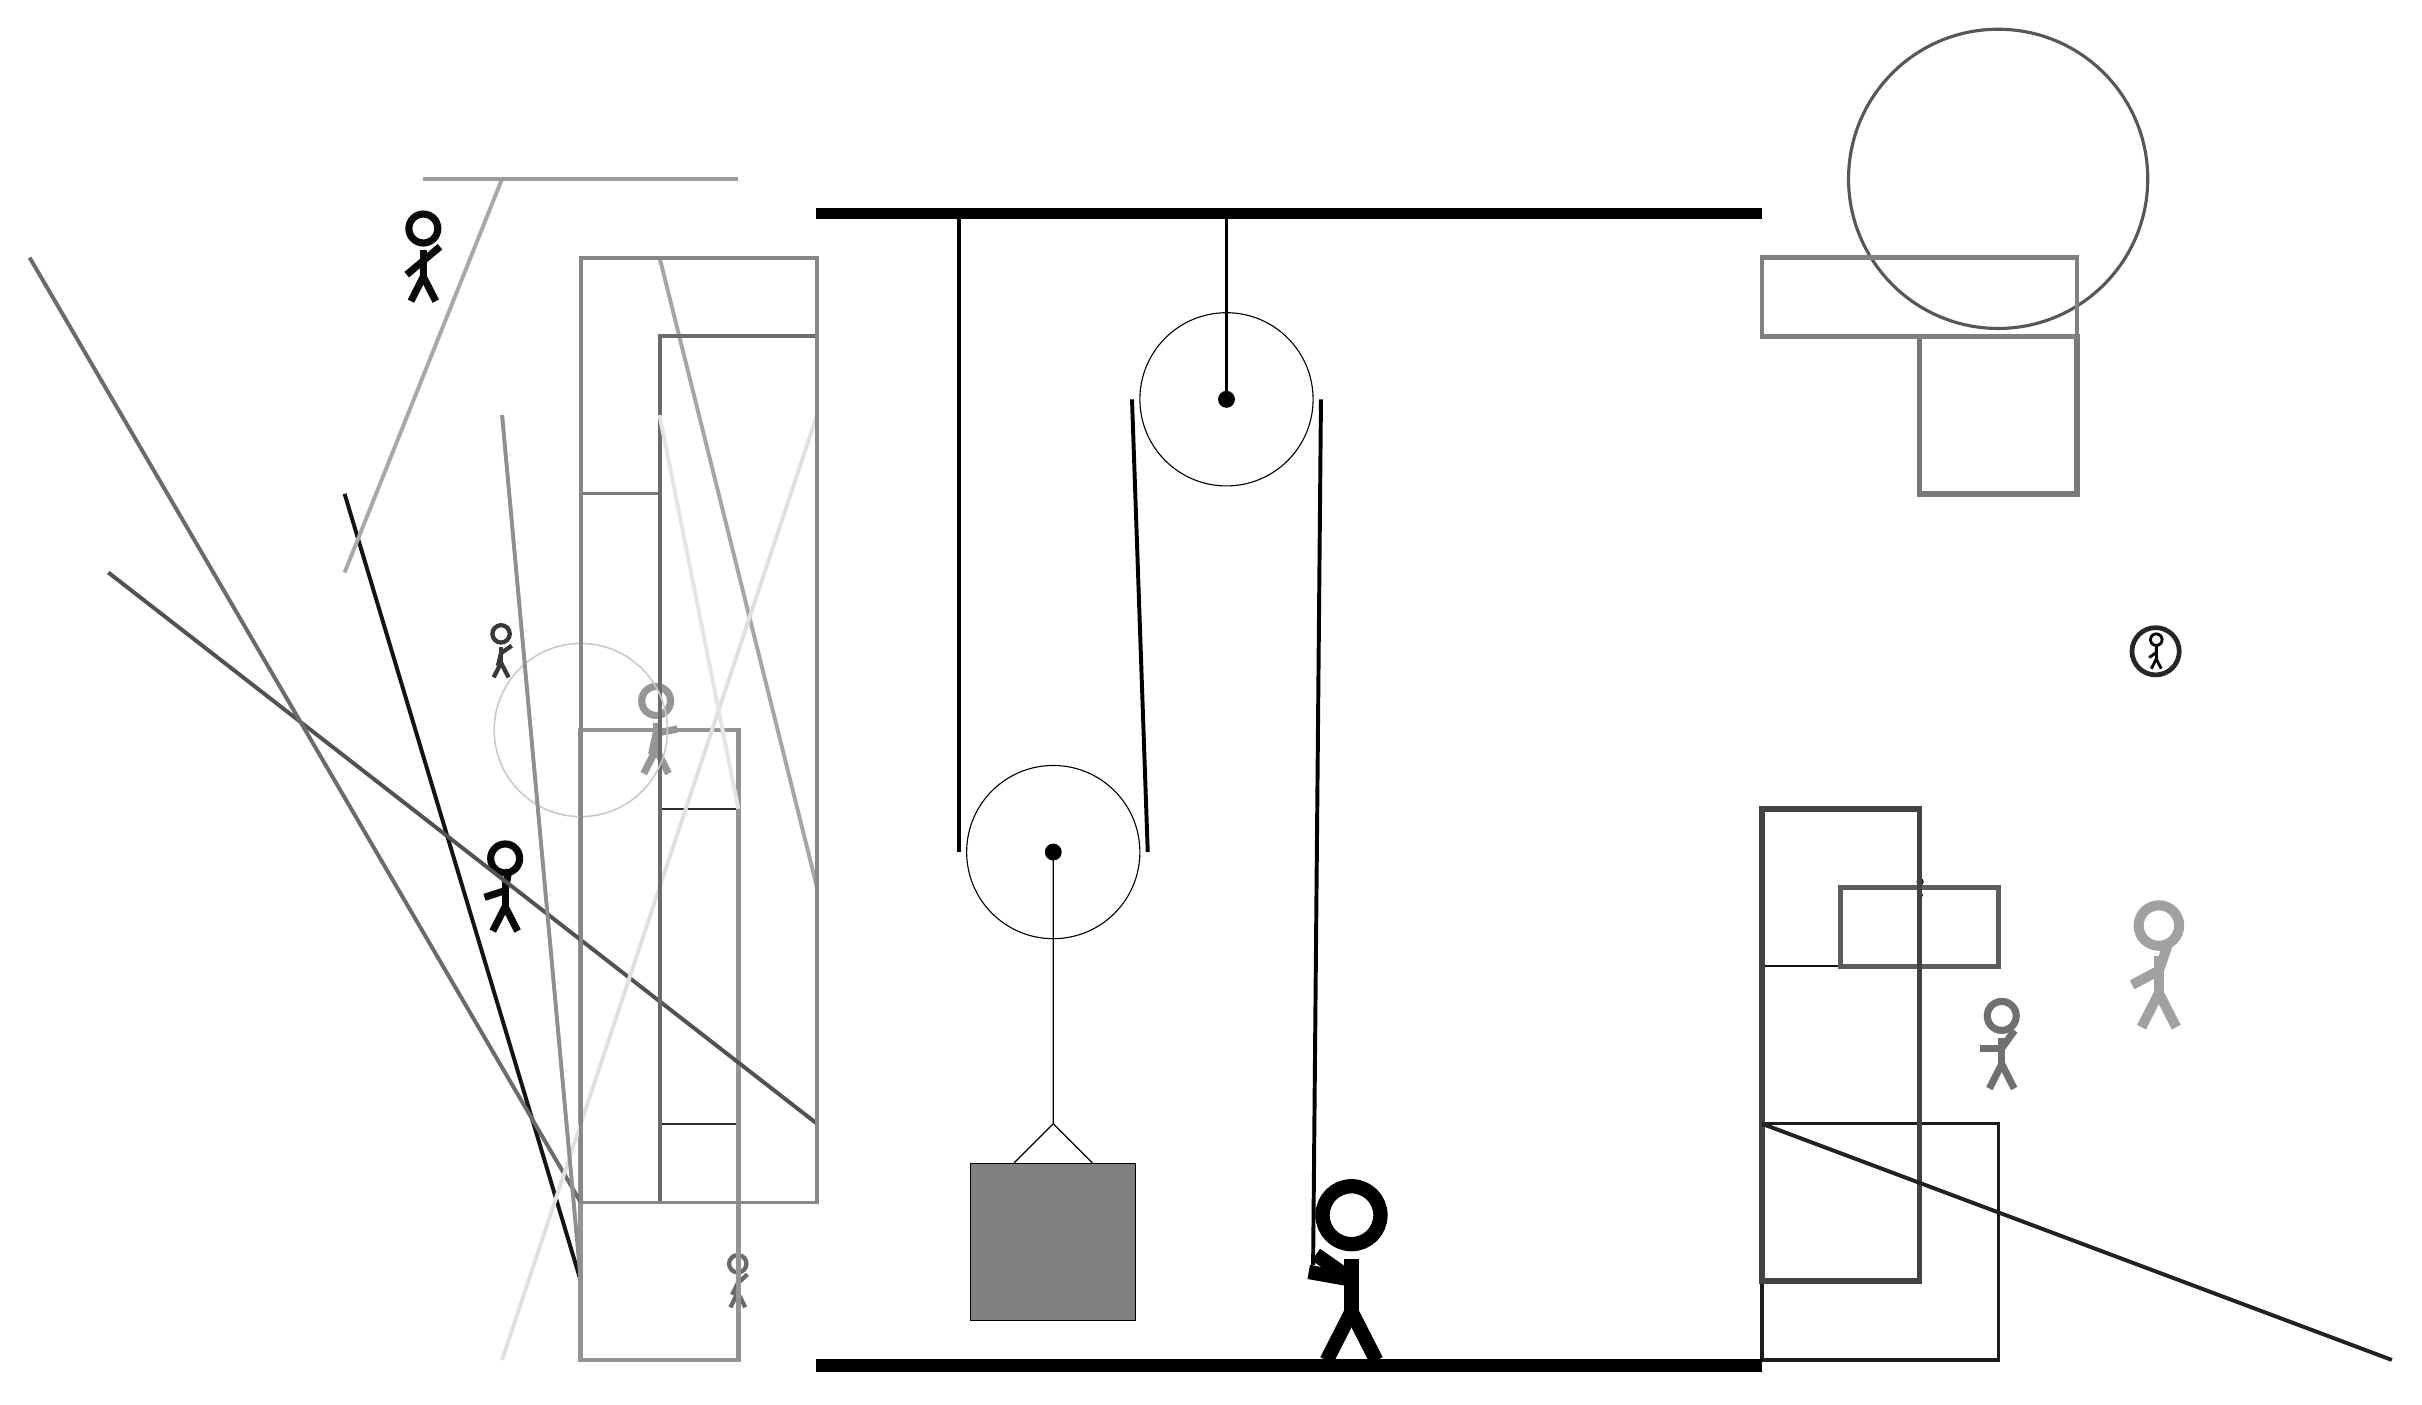
\begin{tikzpicture}
			%%%%% START %%%%%
			
			\draw[fill=black] (-2, 11.5) rectangle (10, 11.625);
			
			\draw (3.2, 9.2) circle (1.1);
			\draw[fill=black] (3.2, 9.2) circle (0.1);
			\draw[thick] (3.2, 9.2) -- (3.2, 11.5);
			
			\draw (1, 3.45) circle (1.1);
			\draw[fill=black] (1, 3.45) circle (0.1);
			
			\draw (1, 3.45) -- (1, 0.0) -- (0.5, -0.5);
			\draw (1, 0.0) -- (1.5, -0.5);
			\draw[fill=black!50] (-0.05, -0.5) rectangle (2.05, -2.5);
			
			\draw[line width=0.5mm, color=black!92](-5, -2) -- (-8, 8);
			
			\node[line width=0.5mm, color=black!78] at (-6, 6) {\Strichmaxerl[3][76][35]};
			\node[line width=0.2mm, color=black!59] at (-3, -2) {\Strichmaxerl[3][64][42]};
			\draw[line width=0.3mm, color=black!82] (-4, 0) rectangle (-3, 4);
			\node[line width=0.5mm, color=black!37] at (15, 2) {\Strichmaxerl[7][28][71]};
			\draw[line width=0.5mm, color=black!34](-6, 12) -- (-8, 7);
			\node[line width=0.6mm, color=black!97] at (-6, 3) {\Strichmaxerl[5][18][80]};
			
			\node[line width=0.3mm, color=black!96] at (-7, 11) {\Strichmaxerl[5][40][40]};
			\draw[line width=0.7mm, color=black!53] (12, 8) rectangle (14, 10);
			\draw[line width=0.4mm, color=black!53] (-4, 8) rectangle (-5, 8);
			
			\draw[line width=0.2mm, color=black!85] (10, 3) rectangle (10, 0);
			\draw [line width=0.6mm, color=black!85](15, 6) circle (0.3);
			\node[line width=0.4mm, color=black!89] at (12, 3) {\Strichmaxerl[1][9][66]};
			\draw[line width=0.5mm, color=black!35](-2, 3) -- (-4, 11);
			\draw[line width=0.6mm, color=black!42] (-3, -3) rectangle (-5, 5);
			\node[line width=0.6mm, color=black!99] at (15, 6) {\Strichmaxerl[2][35][89]};
			
			\draw[line width=0.5mm, color=black!68](-2, 0) -- (-11, 7);
			\draw[line width=0.5mm, color=black!58](-5, -1) -- (-12, 11);
			\draw [line width=0.4mm, color=black!66](13, 12) circle (1.9);
			\node[line width=0.2mm, color=black!41] at (-4, 5) {\Strichmaxerl[5][78][11]};
			\draw[line width=0.5mm, color=black!39](-7, 12) -- (-3, 12);
			
			\draw[line width=0.5mm, color=black!12](-6, -3) -- (-2, 9);
			\draw[line width=0.4mm, color=black!89] (10, -3) rectangle (13, 0);
			\draw[line width=0.2mm, color=black!93] (12, 2) rectangle (10, 4);
			\draw[line width=0.5mm, color=black!58] (-2, -1) rectangle (-4, 10);
			
			\draw[line width=0.6mm, color=black!64] (11, 3) rectangle (13, 2);
			
			\draw[line width=0.6mm, color=black!50] (10, 11) rectangle (14, 10);
			\node[line width=0.7mm, color=black!56] at (13, 1) {\Strichmaxerl[5][0][54]};
			\draw [line width=0.2mm, color=black!21](-5, 5) circle (1.1);
			\draw[line width=0.5mm, color=black!47] (-2, 11) rectangle (-5, -1);
			\draw[line width=0.5mm, color=black!10](-4, 9) -- (-3, 4);
			
			\draw[line width=0.5mm, color=black!44](-5, -2) -- (-6, 9);
			\draw[line width=0.7mm, color=black!74] (12, -2) rectangle (10, 4);
			\draw[line width=0.5mm, color=black!87](10, 0) -- (18, -3);
			
			\draw[line width=0.5mm] (-0.2, 11.5) -- (-0.2, 3.45);
			\centerarc[line width=0.5mm](1, 3.45)(180:360:1.2000000000000002);
			\draw[line width=0.5mm](2.2, 3.45) -- (2.0, 9.2);
			\centerarc[line width=0.5mm](3.2, 9.2)(0:180:1.2000000000000002);
			\draw[line width=0.5mm](4.4, 9.2) -- (4.3, -1.8);
			
			\node at (4.7, -1.9) {\Strichmaxerl[10][-35][170]};
			
			\draw[fill=black] (-2, -3) rectangle (10, -3.15);
			
			%%%%% END %%%%%
		\end{tikzpicture}
	\end{figure}	
\end{document}